
Vơ bản thì cấu trúc của hệ thống nhúng sẽ bao gồm 3 phần: phần mềm hệ thống, phần mềm ứng dụng, bộ vi xử lý.

Phần mềm hệ thống: phần mềm này không bắt buộc phải có và có thể tái sử dụng trên một hệ thống nhúng khác. Chúng có chức năng quản lý bộ nhớ, quản lý tiến trình, quản lý chia sẻ tài nguyên. Trình điều khiển thiết bị: UART, Ethernet, ADC… Hệ điều hành nhúng: eCos, ucLinux, VxWorks, Monta Vista Linux, BIOS, QNX…

Phần mềm ứng dụng: không bắt buộc phải có và khó tái sử dụng trên một hệ thống nhúng khác. Chúng có chức năng quyết định hành vi cho một hệ thống nhúng.

Bộ vi xử lý (Hardware): đây là các thành phần bắt buộc trong một hệ thống nhúng, gồm có một số thiết bị như vi xử lý, bộ nhớ, tụ điện, điện trở, mạch tích hợp, bản in mạch,…

\begin{figure}[H]
	\centering
	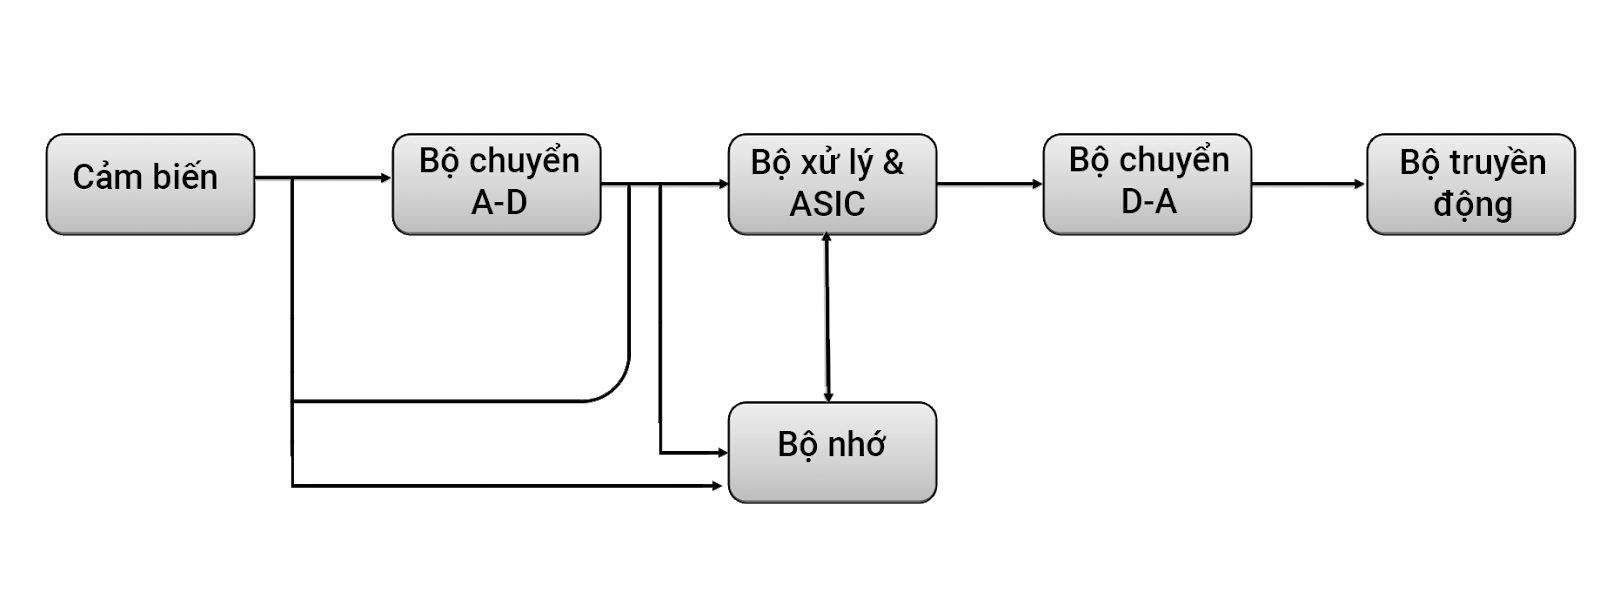
\includegraphics[width=0.8\textwidth]{../images/cau-truc-he-thong-nhung.png}
	\caption{Cấu trúc hệ thống nhúng}
\end{figure}